%!TEX root = informe.tex
\chapter{Antecedentes}\label{cap:antecedentes}

\section{Introducción}\label{sec:introantecedentes}
La mayoría de las ciudades europeas utilizan materiales prefabricados basados en el cemento para urbanizar el terreno transformándolo en espacio público que utilizarán los ciudadanos. Estas instalaciones deben ser resistentes, económicas, funcionales y sobre todo sostenibles. La sostenibilidad es un requisito que ha ido ganando importancia en los últimos años debido no sólo al aspecto económico —costes y mantenimiento principalmente— sino también al medioambiental.

El impacto medioambietal que producen las actividades humanas en la naturaleza debería convertirse en un elemento más de estudio en cualquier proyecto de ingeniería actual. Para el caso de este proyecto, el sector de las obras civiles y urbanismo supone un consumo muy elevado de materias primas y energía —y representa un porcentaje importante del Producto Interior Bruto de España—, lo que implica altas emisiones al medio ambiente \cite{minetur}.

La incorporación de criterios ambientales en la fase de diseño de un producto y/o servicio se denomina \textit{ecodiseño}. El ecodiseño surge como respuesta a la necesidad de introducir estos criterios durante todo el ciclo de vida de un producto con el objetivo de prevenir o reducir su impacto ambiental —principalmente minimizar los residuos, emisiones y costes energéticos \cite{iso14006}. El ecodiseño es el eslabón clave hacia la sostenibilidad y el consumo responsable ya que incorpora nuevos conceptos como la visión de producto-sistema y el ciclo de vida e integra aspectos económicos y sociales como la ecoeficiencia y el ecodiseño sostenible \cite{ihobeeco}.

La metodología del Análisis de Ciclo de Vida (ACV) permite cuantificar todos los procesos relacionados con un producto y/o servicio desde el punto de vista de las \textit{entradas} —materias primas y energía— y \textit{salidas} —emisiones a la tierra, mar o aire y residuos— en el sistema, identificar los puntos clave y establecer una \textbf{estrategia de mejora} \cite{iso14040}.

\begin{figure}[!htb]
\centering
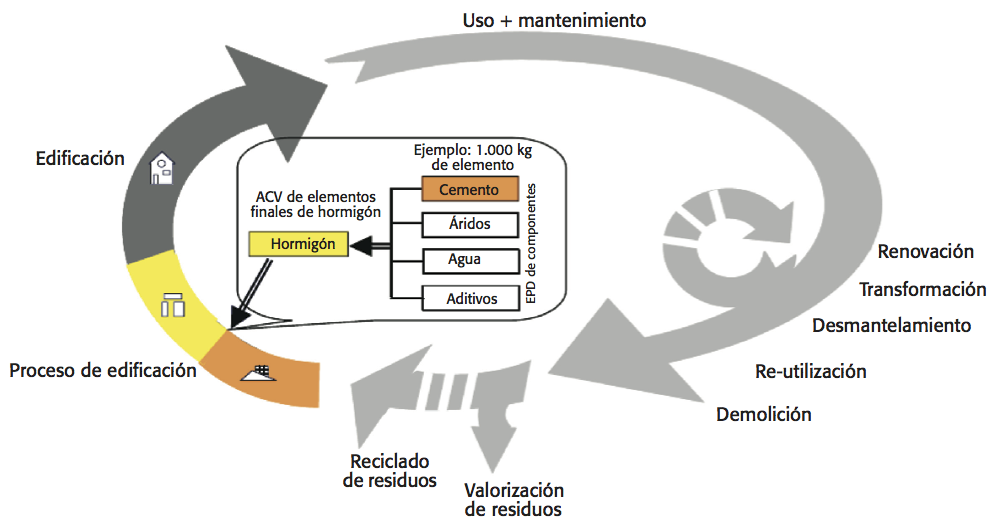
\includegraphics[width=12cm]{img/ciclodevida.png}
\caption[Ciclo de vida de los prefabricados de cemento.]{Ciclo de vida de los prefabricados de cemento. Fuente: \cite{oficemen}.}
\label{fig:ciclodevidaprefabric}
\end{figure}

\section{Relación entre la construcción y el medioambiente}
El sector de la construcción es uno de los más productivos e importantes tanto social como económicamente. Las infraestructuras construidas aportan calidad de vida al ser humano. Como toda actividad humana, el desarrollo de esta actividad provoca impactos significativos en el medio tanto al producir, como al usar y eliminar sus productos \cite{carvalho}.

La concienciación de protección del medio ha obligado al sector a mejorar sus actuaciones en esta materia sin disminuir su capacidad productiva para seguir siendo competitivos. Debe crearse un nuevo paradigma de trabajo en el que el usuario esté satisfecho, el consumo de materia y energía sea mínimo, así como el impacto medioambiental, pero a su vez mejorando la calidad y disminuyendo el tiempo y el coste \cite{augenbroe}.

El impacto medioambiental de un producto cambia según la etapa del ciclo de vida, produciendo diferentes efectos contaminantes sobre el entorno y sobre las personas. Sirvan de ejemplo los siguientes datos \cite{carvalho}:
\begin{itemize}
\item el sector de la construcción moviliza un 10\% de la economía mundial y consume un 40\% de la energía mundial producida cada año.
\item según estudios realizados en varios países europeos entre los que se encuentra España, el consumo energético asociado al sector se distribuye en:
  \begin{itemize}
  \item 19\% para la construcción y mantenimiento de edificios.
  \item 48\% para el consumo directo debido a su uso (electricidad, gas, etc.).
  \item 33\% para el transporte.
  \end{itemize}
  \item los residuos de la construcción y demolición (RCD) generados en la Unión Europea superan los 180 millones de toneladas cada año, es decir, 480 \si{kg} por persona y año. Del total de esos residuos, sólo el 28\% son reutilizados \footnote{Como se indica en la sección \ref{sec:ventajas}, en el caso de los adoquines se recupera el 95\% del total fabricado.}.
\end{itemize}

\section{Descripción del ciclo de vida de un producto de la construcción}
Una buena práctica para poder comprender mejor el ciclo de vida de un producto es la estructuración del sistema en procesos, de forma que queden representados todos los subsistemas constituyentes y se pueda identificar claramente un inicio y un final de cada uno.

El diagrama de la figura \ref{fig:flujo_generico_acv} representa los flujos de entrada (materiales, energía, productos inacabados) y salida (productos finales, productos inacabados, co-productos, residuos) aportando una visión más clara de las fases del ciclo completo. Con los elementos bien identificados es más fácil atribuirle causas y consecuencias tanto a un subsistema como al sistema completo.

\begin{figure}[!htb]
\centering
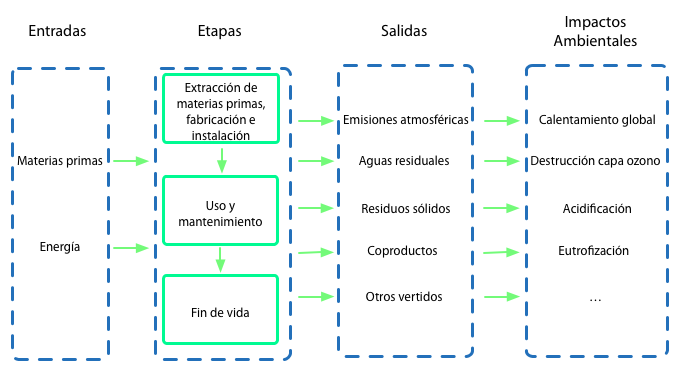
\includegraphics[width=15cm]{img/flujo_generico_acv.png}
\caption[Flujo genérico del ciclo de vida de un producto.]{Flujo genérico del ciclo de vida de un producto. Fuente: elaboración propia basada en \cite{pfullana}.}
\label{fig:flujo_generico_acv}
\end{figure}

\section{Impactos potenciales del adoquín al medio ambiente}
A la hora de analizar los aspecto medioambientales de un sistema es necesario establecer diferentes niveles de análisis para poder seleccionar una estrategia de estudio, ya que a lo largo de la vida de un producto se pueden encontrar diferentes contextos.

\begin{figure}[!htb]
\centering
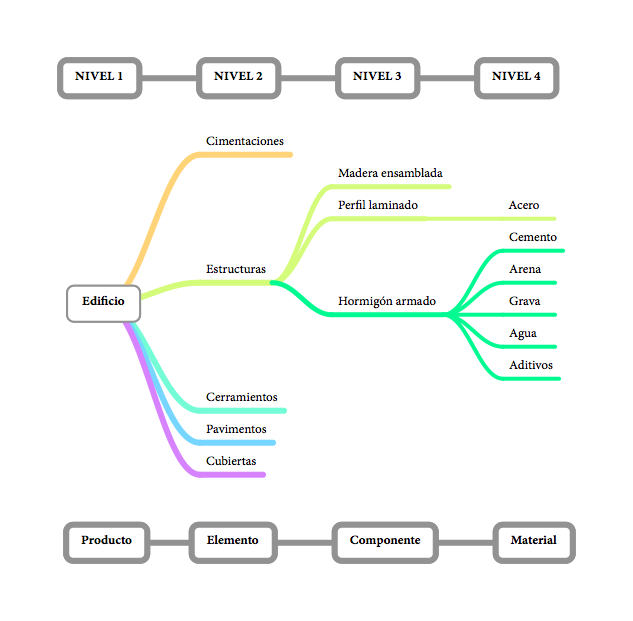
\includegraphics[width=15cm]{img/niveles_productos_construccion.png}
\caption[Niveles de los productos de la construcción.]{Niveles de los productos de la construcción. Fuente: elaboración propia basada en \protect\cite{carvalho}.}
\label{fig:niveles_productos_construccion}
\end{figure}

Al ser el adoquín un elemento de pavimentación se encontraría en el denominado nivel 2 (ver figura \ref{fig:niveles_productos_construccion}). Los impactos medioambientales del nivel 2 se clasifican según el momento de su vida en:

\begin{itemize}
  \item Extracción de materias primas, fabricación e instalación:
    \begin{itemize}
     \item Consumo de energía y recursos naturales en los procesos de extracción de materias primas, fabricación, instalación y transporte.
     \item Producción de ruidos y vibraciones.
     \item Producción de residuos por excedentes de procesos y embalajes.
     \item Emisiones de partículas al aire (p. ej.: polvo).
    \end{itemize}
  \item Uso y mantenimiento:
    \begin{itemize}
      \item Consumo de energía y recursos en los procesos de mantenimiento.
      \item Producción de residuos o sustancias tóxicas en función de los procesos de mantenimiento, su naturaleza y vida útil.
    \end{itemize}
  \item Fin de vida:
    \begin{itemize}
      \item Consumo de energía en el proceso de transporte y reciclaje.
      \item Producción de residuos por la parte no reciclada.
    \end{itemize}
\end{itemize}

\section{Prefabricados del cemento. Adoquines}

\subsection{Historia de los adoquines}
A lo largo de la historia de la humanidad se han ido utilizando diferentes tipos de adoquines para pavimentar los suelos urbanos. Los primeros adoquines eran de piedra, obtenidos a partir de los guijarros de río colocados sobre una capa de arena, usando una mezcla de cal y arena como sellante de juntas  \cite{euroadoquin}.

Debido al coste y el ruido del tráfico rodado, en la primera mitad del siglo XIX comenzaron a usarse los adoquines de madera, utilizando para el sellado residuos bituminosos. Su reducida duración y la posterior aparición de los neumáticos hicieron que los adoquines de madera fueran sustituidos por un modelo cerámico, con el que se usaba la misma arena tanto para la base como sellante.

Los adoquines de piedra iniciales seguían siendo más resistentes y además no eran tan deslizantes como los cerámicos. A finales del siglo XIX se fabricó por primera vez el \textbf{adoquín de hormigón}. Estos adoquines proporcionaban una mayor uniformidad que los de piedra, eran muy resistentes y con un coste inferior. Alemania y Países Bajos fueron los primeros en incorporar este nuevo formato de adoquín a sus núcleos urbanos. Al principio se usaban modelos que imitaban a los de piedra tanto en forma como colocación, pero pronto se añadieron formas dentadas o curvas, permitiendo una mejor alineación con el trazado.

Finalmente, durante la década de los 70 se mejoraron sustancialmente los sistemas de fabricación, permitiendo una gran variedad de modelos de adoquines y un abaratamiento de los costes de fabricación e instalación que llega hasta nuestros días.

\subsection{Ventajas e inconvenientes del uso de adoquines}\label{sec:ventajas}

En comparación con otros tipos de pavimentos tales como los asfálticos o los pavimentos contínuos hormigonados, los adoquines presentan las siguientes ventajas:

\begin{itemize}
\item Fabricación: no se utilizan derivados del petróleo, que suelen ser caros y contaminantes, además de requerir una mayor aportación de energía durante el proceso de fabricación. En contraposición, pueden utilizarse cementos y áridos locales, disminuyendo los costes de transporte.

El proceso de fabricación de los adoquines requiere una maquinaria específica debido a que son sometidos a presión y vibración para segurar una resistencia y durabilidad adecuadas. Esto implica un control sobre la fabricación, consistencia y fiabilidad del producto mayor que el resto de pavimentos.

\item Instalación: aunque los adoquines pueden colocarse de forma automatizada, están diseñados de base para ser colocados manualmente, permitiendo instalarse en zonas de difícil acceso, cargas elevadas (muelles de carga, aeropuertos, \ldots), resolver trazados complejos o pendientes pronunciadas. A diferencia de los pavimentos asfálticos, su ejecución no depende de la temperatura ambiente y pueden ser utilizados inmediatamente después de su finalización, lo que implica una reducción en los tiempos de ejecución de obra.

\item Comportamiento: los adoquines pueden ser diseñados para ser muy resistentes tanto a cargas verticales (distribuidas o puntuales) como a esfuerzos horizontales (aceleración-frenada, giros,\ldots). Además, soportan bien sin degradarse los vertidos de aceites y combustibles sobre el pavimento. Los niveles de ruido generados por el tráfico son similares o inferiores a otros pavimentos en ausencia de humedad y sensiblemente inferiores en condiciones de humedad, especialmente a bajas velocidades. La resistencia a deslizamiento es mayor al del resto de pavimentos.

\item Mantenimiento: la vida útil del adoquín viene determinada principalmente por el comportamiento de la base, subbase y explanada y no por el propio adoquín. La vida útil \footnote{La vida útil se considera como la duración estimada que un objeto puede tener cumpliendo correctamente con la funcion para la cual ha sido creado.} de cálculo suele ser a 30 años, aunque en condiciones normales puede superar los 50 años. De esta manera, al renovar el pavimento se puede reutilizar un 95\% de los adoquines originales \cite{euroadoquin}. El adoquín es la mejor opción en zonas donde aún no se han implantado todos los servicios de públicos debido a que pueden ser levantados fácilmente para llevar tareas de instalación o reparación en el subsuelo. La conservación de los adoquines se limita al relleno de juntas erosionadas con arena de sellado cada cierto tiempo y a la reposición de adoquines fracturados.

\item Costes: aunque inicialmente el precio del metro cuadrado instalado es algo superior a otros pavimentos, a largo plazo es mucho más barato debido al menor mantenimiento y la reutilización de piezas. Los pavimentos asfálticos y hormigonados requieren un mayor esfuerzo e inversión a la hora de ser reparados o retirados para acceder al subsuelo \cite{pavimentos,euroadoquin}.

\item Aspecto estético: actualmente los adoquines pueden diseñarse de todas formas, texturas, colores y disposiciones según las necesidades de la obra.
\end{itemize}


Realmente el uso de adoquines apenas tiene inconvenientes, aunque existen varios, entre los que destacan:

\begin{itemize}
  \item Incomodidad: debido a que el pavimento está lleno de juntas de separación entre adoquines y poco a poco se vuelve irregular, la circulación y el paso pueden ser incómodos y conllevar mayores costes de operación a los vehículos.
  \item Nieve: el pavimento de adoquines suele ser irregular y no permite bien la retirada de nieve en zonas con climas donde nieva mucho. Por otro lado, la nieve se derrite antes en pavimentos de asfalto, de color negro, debido al calentamiento del sol.
\end{itemize}

\section{Materias primas de los prefabricados del cemento}
Las características de las materias primas que se pueden emplear en la fabricación de los adoquines se contemplan en la norma UNE-EN 1338:2004/AC:2006 \cite{une1338}. En ella se especifican detalladamente los materiales, propiedades, requisitos y métodos de ensayo de los adoquines prefabricados de hormigón no armados y accesorios complementarios, previstos para uso peatonal, uso en áreas sometidas a tráfico de vehículos y cubiertas, como por ejemplo: aceras, límites de áreas, sendas para bicicletas, aparcamientos, carreteras, autopistas, áreas industriales, aeropuertos, estaciones de autobuses y gasolineras. Esta norma no trata la visibilidad y la tactibilidad de los adoquines ni los adoquines permeables.

\subsection{Cemento}
El cemento es un conglomerante formado a partir de arcilla y caliza (\ce{CaCO3}), que se endure al mezclarse con agua. Para producir cemento (ver figura \ref{fig:cemento}), la arcilla y la caliza se muelen juntas. A esta mezcla se le añade yeso para conferirle la propiedad de fraguar y endurecerse. El resultado se introduce en un horno rotatorio, normalmente seco por ser más eficiente energéticamente, a una temperatura aproximada de 1450\si{\celsius}. A continuación se introduce el material en un incinerador donde el calentamiento produce la liberación del \ce{CO2} de la caliza y se produce el cemento \emph{clinker}.

\begin{center}
\ce{CaCO3 + calor -> CaO + CO2}
\end{center}

El clinker es el óxido de calcio (\ce{CaO}) obtenido de la reacción anterior, que puede encontrarse acompañado de otros minerales como hierro, aluminio o silicio. El aporte de calor necesario para obtener el clinker representa la mayor parte del coste energético en la producción de cemento.

Por último, se produce la molienda del clinker junto con yeso y otros materiales (bauxita, arena,\ldots) para mejorar sus propiedades, produciendo el cemento.

\begin{figure}[!htb]
\centering
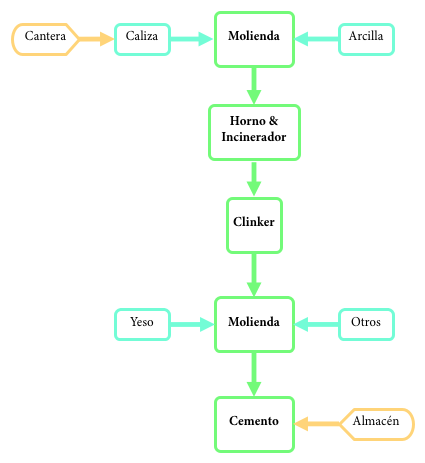
\includegraphics[height=10cm]{img/cemento.png}
\caption[Diagrama de flujo de la fabricación del cemento.]{Diagrama de flujo de la fabricación del cemento. Fuente: elaboración propia basada en \protect\cite{jsjunnesson}.}
\label{fig:cemento}
\end{figure}

Cuando se utiliza la palabra \emph{cemento} se refiere normalmente al cemento tipo Portland —supone un 95\% de la producción de cementos—, nombre no comercial que implica un proceso de producción y una composición característicos \cite{jsjunnesson}. De acuerdo a la norma UNE-EN 197-1:2011 \cite{une1971}, el cemento se divide en tres grupos en función de la cantidad de cemento Portland incluido: CEM I, CEM II y CEM III. El CEM I (95\% a 100\% de contenido de cemento Portland) es el más usado en la fabricación de adoquines.

Con respecto a la normativa específica de adoquines, la norma UNE 80301:1996 \cite{une80301} en el ámbito de España establece los requisitos que debe tener el cemento común. Si se utilizan cementos especiales se recurrirá a la norma UNE 80303:2013, y si son blancos a la norma UNE 80305:2012.

\subsection{Áridos}
Los áridos (entre los que se incluye la arena) son partículas de roca que pueden ser tanto gravas (piedras de forma natural) como macadán (piedras trituradas), teniendo cada tipo una textura diferente (figura \ref{fig:aridosnaturalesytriturados}). Se pueden añadir diferentes tamaños de áridos para ejercer una función específica según el tipo. Fracciones menores rellenarán las cavidades que haya entre partículas mayores, aportando adherencia a costa de un mayor peso.

\begin{figure}[!htb]
\centering
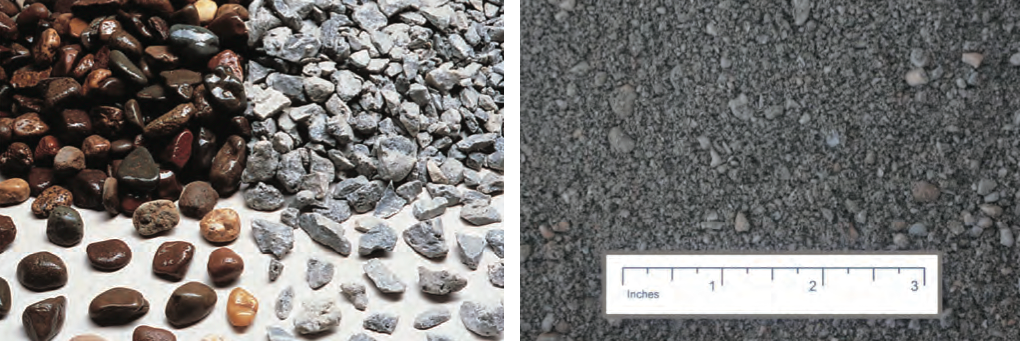
\includegraphics[width=13cm]{img/aridos.png}
\caption[Áridos naturales y triturados. Granulometrías.]{Áridos naturales y triturados. Granulometrías. Fuente: \cite{sustpave}.}
\label{fig:aridosnaturalesytriturados}
\end{figure}

El material de machaqueo para la producción de macadán se criba para eliminar las partículas menores. Debido a que las partículas que forman el macadán son más irregulares, es más fiable como material de relleno por su capacidad de incrustamiento (la grava tiene una forma más redondeada). El macadán puede ser utilizado de forma más generalizada en función de la localización ya que la grava natural es un recurso más limitado.

La fuente de recursos de áridos son principalmente de río, mina o cantera o piedras trituradas (macadán). La granulometría de los áridos que se utilicen deberá cumplir las características indicada en la norma UNE-EN 1338:2004/AC:2006 \cite{une1338}.

\subsection{Agua}
El agua es muy importante en la constitución del hormigón. Reacciona químicamente con el cemento —hidratación— para proporcionar las propiedades deseadas del hormigón \cite{nrmca}. El agua de amasado es la cantidad de agua que toma contacto con el cemento y se usa para determinar las proporciones del resto de elementos para formar la mezcla. La fuerza y la durabilidad del cemento viene dado en gran parte por la cantidad de agua.

Además de su cantidad, la calidad del agua utilizada tiene efectos importantes en las propiedades del hormigón fresco, tales como el tiempo de fraguado y la facilidad de trabajo. También tiene importancia en la fuerza y durabilidad del hormigón endurecido.

\subsubsection{Fuentes posibles de agua}

Por norma general el agua adecuada para el consumo humano —agua potable— es válida. No obstante, el agua no potable puede ser utilizada siempre que no tenga un impacto negativo en las propiedades del hormigón. La mayoría de las plantas tienen una fuente de agua municipal que proporciona agua potable sin necesidad de pruebas de calidad. En zonas rurales o en plantas portátiles in situ —instaladas y desinstaladas en el propio lugar del proyecto—, se suelen utilizar fuentes de agua no potable como ríos o masas de agua.

Otra fuente de agua es la reciclada de la limpieza —agua de lavado— de la mezcladora y otros elementos de la planta. También se podrá aprovechar el agua de precipitaciones atmosféricas que pueda recolectarse en las instalaciones de la planta.

El agua de procesado no sólo se genera de la fabricación del hormigón, sino también del lavado del hormigón reciclado. Los sistemas de recolección procesan el agua con el cemento y los áridos en forma de lechada que puede ser también utilizada como agua para la mezcla de hormigón.

Las normativas medioambientales suelen requerir que las plantas de fabricación traten y procesen tanto el agua de lluvia como el de procesado —agua de operaciones— para que adquiera ciertos niveles de pH y contenidos sólidos antes de que abandonen las instalaciones \cite{ermco}.

\subsubsection{Cualificación del agua no potable}
El agua es el recurso más importante para el ser humano. En algunas zonas el suministro de agua potable es muy escaso. El uso de fuentes de agua no potables para la producción de hormigón mantiene una producción sostenible de hormigón conservando los recursos de agua potable. La gestión del agua procedente de la producción de hormigón conforme con las normativas medioambientales representa un coste adicional para el fabricante, por lo que el uso de agua no potable representa un ahorro considerable en la producción de hormigón. Cuando se utilizan fuentes de agua no potable es importante verificar y documentar que las impurezas que contiene no merman las características del hormigón, ya que las fuentes pueden contener aceites, grasas, sales disueltas y otros elementos no controlados. Por esta razón, el fabricante debería tener en cuenta que su uso implica un coste adicional que evaluar y controlar.

\subsection{Aditivos}
Se podrán utilizar adiciones o aditivos siempre que produzcan el efecto deseado (acelerante, retardante,\ldots) y no afecte a las características esperadas del hormigón.

\section{Consideraciones de la instalación de pavimentos de adoquines}
La correcta colocación y mantenimiento del pavimento con adoquines es igual de importante que la calidad en los materiales y los procesos de fabricación \cite{euroadoquinc} para que el funcionamiento del pavimento sea el adecuado.

Hay múltiples manuales y guías técnicas que explican los criterios prácticos y recomendaciones para una correcta colocación de los adoquines.

La planificación del trabajo empieza estudiando el tipo de vía y uso principal al que estará destinado el pavimento. Una vez decidido es necesario preparar la explanada y las diferentes capas componentes en función de ese uso. A continuación se coloca la capa de adoquines, se sella con arena y se realiza un vibrado del pavimento. Por último se realiza una limpieza final.

\subsection{Capas componentes}

El pavimento de adoquines está compuesto por hasta un máximo de seis capas, cuyas dimensiones y composición dependerán del uso destinado de la vía:

\begin{itemize}
\item Explanada: terreno natural adecuadamente compactado hasta alcanzar una capacidad portante mínima.
\item Subbase: conjunto de capas naturales, de material granular seleccionado, estabilizado y compactado, situadas directamente sobre la explanada.
\item Base: principal elemento portante de la estructura, situada sobre la subbase. Puede ser realizada con material granular, zahorra artificial, con un mayor grado de compactación que el alcanzado en la subbase —base flexible—, o estar realizada con hormigón magro —base rígida.
\item Lecho de árido: base de apoyo de los adoquines, destinada a absorber sus diferencias de espesor debidas a la tolerancia de fabricación, de manera que estos una vez compactados formen una superficie homogénea.
\item Adoquines: elementos prefabricados de hormigón, cuya cara exterior, una vez colocados, forman la capa de rodadura de la superficie a pavimentar.
\item Relleno final: una vez encastrados en el lecho de árido, sus juntas precisan un relleno final para transferir a los elementos contiguos las cargas a las que sean sometidos por acción del tráfico.
\end{itemize}

\subsection{Determinación de la sección tipo}\label{sec:secciontipo}

Se consideran los siguientes casos:

\begin{enumerate}
\item Viales y zonas de aparcamiento\footnote{No suelen existir zonas peatonales puras. Siempre se contemplará el paso eventual de vehículos de mantenimiento, limpieza y servicios.}.
\item Zonas industriales.
\end{enumerate}

Para cada caso, viales o zonas industriales, la sección puede obtenerse de forma abreviada en función de dos variables:
\begin{itemize}
\item Tipo de explanadas.
\item Categoría de tráfico.
\end{itemize}

\subsubsection{Tipo de explanada}

Se utiliza un sistema de clasificación de su capacidad portante mediante el índice CBR (California Bearing Ratio), indicando el tanto por ciento de la presión ejercida por un pistón sobre el suelo para alcanzar una determinada penetración baremado según un juego de muestras normalizados (ver tabla \ref{indicecbr}).

\begin{table}[!htb]
\centering
\begin{tabular}{cc}
\toprule
Calidad de la explanada & Índice CBR\\
\midrule
E1 & 5 $\leq$ CBR = 10\\
E2 & 10 $\leq$ CBR = 20\\
E3 & 20 $\leq$ CBR\\
\bottomrule
\end{tabular}
\caption[Índice CBR.]{Índice CBR. Fuente: \protect\cite{euroadoquinc}.}
\label{indicecbr}
\end{table}


\subsubsection{Categoría de tráfico}

\begin{table}[!htb]
\centering
\begin{tabular}{cc}
\toprule
Tipo & Categoría de tráfico\\
\midrule
Viales y zonas de aparcamiento & C0 \ldots C4\\
Zonas industriales & A \ldots D\\
\bottomrule
\end{tabular}
\caption[Categoría de tráfico.]{Categoría de tráfico. Fuente: \protect\cite{euroadoquinc}.}
\label{categoriadetrafico}
\end{table}

Si en un área limitada existen diversos usos, a efectos de unificación se debería emplear para toda la zona la carga de cálculo más exigente.

\begin{table}[!htb]
\centering
\begin{tabular}{p{7cm}c}
\toprule
Uso previsto & Categoría de tráfico\\
\midrule
Arterias principales con gran afluencia de tráfico, paradas de bus, estaciones de servicio, etc. (50 a 149 v.p.d.) & C0\\
Arterias principales (25 a 49 v.p.d.) & C1\\
Calles comerciales con gran actividad (16 a 24 v.p.d.) & C2\\
Calles comerciales cone escasa actividad (15 v.p.d.) & C3\\
Áreas peatonales, calles residenciales & C4\\
\bottomrule
\end{tabular}
\caption[Categoría de tráfico en viales y zonas de aparcamiento.]{Categoría de tráfico en viales y zonas de aparcamiento. Fuente: \protect\cite{euroadoquinc}.}
\label{categoriadetraficoenviales}
\end{table}

\begin{table}[!htb]
\centering
\begin{tabular}{cccc}
\toprule
\multicolumn{2}{c}{Área} & Uso & Intensidad de uso\\
\midrule
\multirow{7}{*}{Comercial} & De operación & — & Alta\\
& \multirow{2}{*}{Almacenamiento} & Mercancia convencional & Media\\
& & Mercancía pesada & Alta\\
& Manipulación & — & Alta\\
& \multirow{3}{*}{Estacionamiento} & Vehículos pesados y ligeros & Media\\
& & Vehículos pesados exclusivamente & Alta\\
& & Semirremolques & Alta\\
\midrule
\multirow{3}{*}{Militar} & De operación & — & Alta\\
& \multirow{2}{*}{Almacenamiento} & Mercancia convencional & Media\\
& & Mercancía pesada y semirremolques & Alta\\
\midrule
\multirow{3}{*}{Pesquera} & Almacenamiento & — & Media\\
& Manipulación & — & Alta\\
& Clasificación y venta & — & Media\\
\midrule
\multirow{3}{*}{Industrial} & De operación & — & Alta\\
& \multirow{2}{*}{Almacenamiento} & Mercancia convencional & Media\\
& & Mercancía pesada & Alta\\
\bottomrule
\end{tabular}
\caption[Intensidades de uso en zonas industriales.]{Intensidades de uso en zonas industriales. Fuente: \protect\cite{euroadoquinc}.}
\label{categoriadetraficoenzonasindustrialesintensidades}
\end{table}

\begin{table}[!htb]
\centering
\begin{tabular}{cccc}
\toprule
Intensidad de uso & \multicolumn{3}{c}{Carga de cálculo}\\
\cmidrule{2-4}
& Alta & Media & Baja\\
\midrule
Elevada & A & B & C\\
Media & A & B & D\\
Reducida & B & C & D\\
\bottomrule
\end{tabular}
\caption[Categoría de tráfico en zonas industriales.]{Categoría de tráfico en zonas industriales. Fuente: \protect\cite{euroadoquinc}.}
\label{categoriadetraficoenzonasindustriales}
\end{table}

\subsection{Secciones tipo}

Las secciones tipo según la base y el uso previsto del área vistas en la sección \ref{sec:secciontipo} pueden resumirse en cinco tipos para cada tipo de base, granular (figura \ref{fig:seccionestipogranular}) u hormigón magro (figura \ref{fig:seccionestipohormigon}).

\begin{figure}[!htb]
\centering
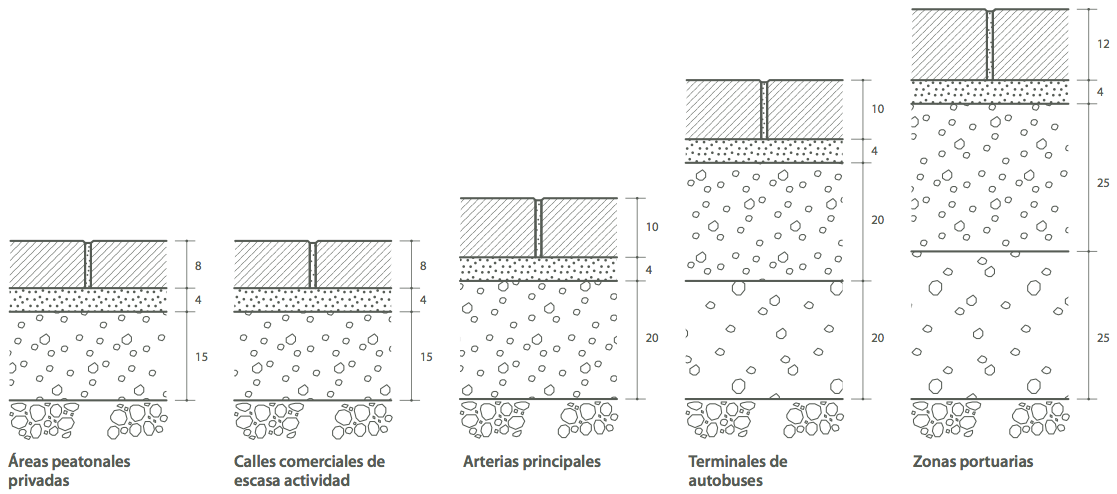
\includegraphics[width=15cm]{img/seccionestipo_1.png}
\caption[Secciones tipo para base granular.]{Secciones tipo para base granular. Unidades en cm. Fuente: \cite{fenollar}.}
\label{fig:seccionestipogranular}
\end{figure}

\begin{figure}[!htb]
\centering
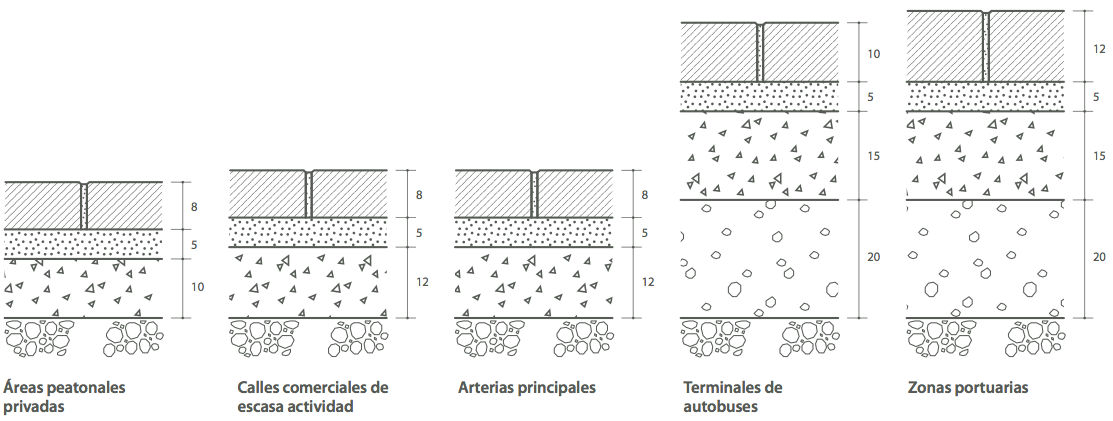
\includegraphics[width=15cm]{img/seccionestipo_2.png}
\caption[Secciones tipo para base de hormigón.]{Secciones tipo para base de hormigón. Unidades en cm. Fuente: \cite{fenollar}.}
\label{fig:seccionestipohormigon}
\end{figure}

\section{Consideraciones para el uso y mantenimiento de pavimentos de adoquines}\label{sec:consideracionesuso}

Una de las principales ventajas del pavimento con adoquines de hormigón es el fácil y económico mantenimiento del mismo durante su vida útil. Aunque la esperanza de vida de un adoquín está probada en 50 años, su tiempo de diseño es únicamente 30 años \cite{euroadoquin}.

Para que el funcionamiento del pavimento sea el correcto, las juntas deben permanecer llenas de arena —la presencia de pasto en las juntas no es nociva—. Si se pierde más de 1 \si{cm} de sello se recomienda corregir el hueco con arena de sellado.

Si se hunde el pavimento o es necesario acceder a infraestructura urbana, se deben retirar los adoquines, realizar la reparación y volver a reconstruir la franja de pavimento. La presencia de ondulaciones en la superficie del pavimento puede ser un indicio de que fue construido con una base mal construida o las características del tráfico no son las de diseño.

El pavimento de adoquines debe limpiarse, en principio, únicamente por barrido. El lavado con manguera debe ser poco frecuente y sólo cuando el tamaño de las juntas sea pequeño.

Existe un mantenimiento periódico, cada 3-5 años, que consiste en renovar el sellado del pavimento debido a la acción erosiva del medio ambiente \cite{malaka}.

\section{Consideraciones para el fin de vida del adoquín}\label{sec:consideracionesfindevida}

\subsection{Introducción}

La finalidad del reciclaje es conseguir un objetivo de cero residuos utilizando todos los materiales de subproductos encontrados en la rehabilitación o reconstrucción del pavimento. Esto no es sólo una ventaja económica, sino que el reciclaje local minimiza el impacto medioambiental reduciendo la huella de carbono, la energía utilizada y las emisiones, además de reducir la necesidad de vertederos y la extracción de materias primas no renovables.

El concepto del reciclaje debe verse como un proceso de ``cuna a cuna'' en contraposición al pensamiento de ``la cuna a la tumba'' de hace unos años. En la práctica no hay una tumba para los materiales utilizados en las infraestructuras sostenibles actuales, tan sólo un nuevo inicio que permite la aplicación de tecnologías para lograr la meta de cero residuos en la rehabilitación y reconstrucción de pavimentos de adoquines.

Mientras que en el pasado los costes económicos eran el factor prioritario que empujaban al reciclaje, actualmente se tienen en cuenta los recursos limitados y la conciencia medioambiental en beneficio de la sostenibilidad en el proceso. Aunque el coste económico sigue siendo un factor importante, la concienciación política y social de la necesidad de ser sostenible ha aumentado considerablemente en los últimos años \cite{sustpave}. Los beneficios del reciclaje incluyen:

\begin{itemize}
  \item ahorros económicos.
  \item menor uso de materias primas no renovables.
  \item menor demanda de combustibles y emisiones asociadas del transporte de desechos a vertederos o de nuevos materiales a su destino.
  \item mejora del uso del suelo municipal, minimizando tanto la necesidad de vertederos como de nuevos espacios para la extracción de recursos.
\end{itemize}

Se generan aproximadamente 200 millones de toneladas de Residuos de la Construcción y Demolición (RCDs) al año en Europa. El hormigón es un material de construcción excelente para edificios energéticamente eficientes y duraderos. Por suerte, además puede reciclarse con un impacto medioambiental mínimo \cite{europeanconcrete}.

\subsection{Reciclado del hormigón}

En la actualidad, el hormigón —cemento, áridos, arena y agua— recuperado de los RCDs no puede utilizarse para obtener de nuevo cemento. En su lugar, ese hormigón puede ser machacado y utilizado como árido para formar parte de nuevas estructuras, principalmente formando bases de carreteras, aunque cada vez más nuevo hormigón usando un porcentaje de hormigón reciclado. Se puede utilizar árido reciclado hasta un máximo de un 20\% del total necesario en la fabricación de nuevo hormigón conservando las propiedades originales \cite{europeanconcrete}.

El hormigón machacado se utiliza principalmente en obras de construcción, carreteras, calles y aparcamientos, aunque también como relleno de excavaciones de tuberías y cimientos de edificios. El hormigón reciclado en forma de árido reciclado tiene frecuentemente mejor grado de compacidad y densidad y es normalmente más barato que el material original \cite{jsjunnesson}.

El proceso de reciclado suele consistir en que el RCD llega a la planta de reciclaje, donde es introducido en una tolva de recepción, protegida con una reja de filtrado para la eliminación de los materiales de gran tamaño. El residuo es conducido por un sistema de cintas para su clasificación y triaje. Finalmente se produce un machacado seguido de un lavado-secado y un tamizado \cite{monografia} \cite{gerd}.

En el caso concreto de los adoquines, su fin de vida se puede desglosar en dos escenarios \cite{euroadoquin}:
\begin{itemize}
  \item el 95\% de los adoquines son recuperados para su reciclaje;
  \item el 5\% son desechados en vertederos junto con otros residuos.
\end{itemize}

El reciclado puede tratarse como un beneficio para el medio ambiente, debido a que se evita extraer nuevas materias primas. Ese beneficio se obtiene como la diferencia entre los impactos de las nuevas materias primas y los impactos del proceso de reciclaje.

El reciclado del hormigón en nuevos áridos implica que habrá un \textbf{producto evitado}, que ya no es necesario fabricar, que será el propio árido. que además será coincidente con el \textbf{producto secundario}, que es el obtenido después del proceso de reciclaje.

\section{Origen del estudio}
Malaka de Prefabricados es una empresa malagueña que inició su actividad en 1994. Su compromiso consistía en integrarse en el tejido industrial de la provincia, estableciendo lazos con otras industrias locales, y apostar por un producto de calidad que marcara la diferencia en el mercado sin repercutir en el precio.

\begin{figure}[!htb]
\centering
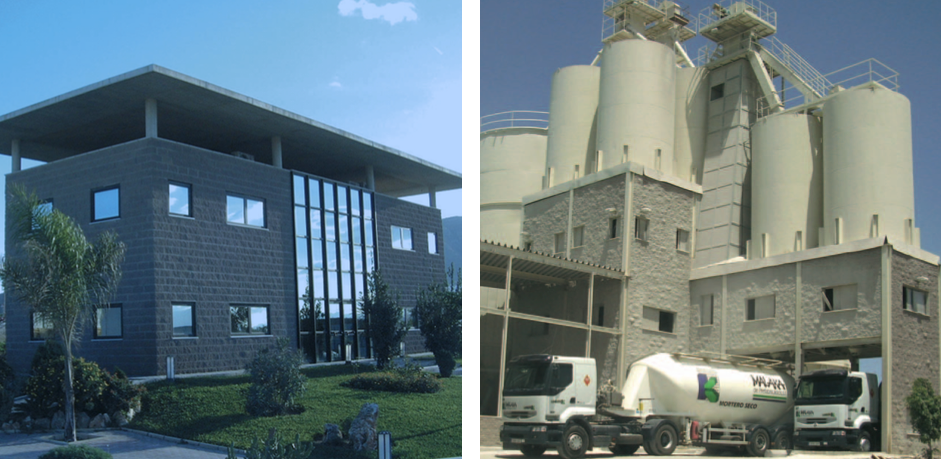
\includegraphics[width=15cm]{img/malaka1.png}
\caption[Instalaciones de Malaka de Prefabricados.]{Instalaciones de Malaka de Prefabricados. Fuente: \protect\cite{malakacatalogo}.}
\label{fig:malakainstalaciones1}
\end{figure}

A finales de la década de los 90 y principios del nuevo milenio experimentaron un fuerte crecimiento como consecuencia del rápido auge del sector de la construcción en Andalucía, convirtiéndose en un referente de los prefabricados en la provincia y en la comunidad autónoma.

Sus principales líneas de producción son los adoquines, bloques y bordillos de hormigón, a los que se dedica por completo una planta de producción automatizada. La línea de adoquines dispone de varias gamas de producto debido a la versatilidad y demanda de la que disfruta. El resto de productos —tubos, registros, aligerantes, casetones y mortero seco ensilado— se fabrican en la segunda planta.

\begin{figure}[!htb]
\centering
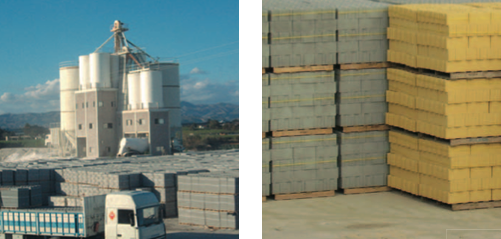
\includegraphics[width=15cm]{img/malaka2.png}
\caption[Instalaciones accesorias de Malaka de Prefabricados.]{Instalaciones accesorias de Malaka de Prefabricados. Fuente: \protect\cite{malakacatalogo}.}
\label{fig:malakainstalaciones2}
\end{figure}

El compromiso de calidad en sus productos pasó por cumplir todos los requisitos de la normativa española y europea, adoptando el marcado CE como sello de calidad. Tanto clientes como partners pueden dar muestra de su confianza en la calidad de los mismos. Entre sus principales proyectos se encuentran el Palacio de Deportes Martín Carpena (Ferrovial-Agroman), el Parque Temático de Melilla (Dragados) y colaboraciones con los ayuntamientos de Marbella y Estepona.

Durante los casi veinte años en la industria han intentado adoptar las mejores y más novedosas tecnologías de fabricación del sector, ampliando de forma progresiva el tamaño de sus instalaciones en la Finca Pizarro, a las afueras de la ciudad de Málaga.

La empresa adoptó a principios de 2000 la Certificación de Sistemas de Gestión de la Calidad (ISO 9001) y varios años más tarde la Certificación Sistemas de Gestión Ambiental (ISO 14000) como referente de compromiso con la calidad de su producción y con el medioambiente.
